% === Figure: CPA precision-from-Steiner bar ================================
% CONFIRMED: threshold decode P = 0.761 ; arborescence/Steiner decode P = 0.805.
%   Recall is ~equal (0.578 vs 0.582), so the global-consistency constraint buys
%   precision. Same per-link scores for both decoders -> clean ablation.
% Standalone-includable: % === Figure: CPA precision-from-Steiner bar ================================
% CONFIRMED: threshold decode P = 0.761 ; arborescence/Steiner decode P = 0.805.
%   Recall is ~equal (0.578 vs 0.582), so the global-consistency constraint buys
%   precision. Same per-link scores for both decoders -> clean ablation.
% Standalone-includable: % === Figure: CPA precision-from-Steiner bar ================================
% CONFIRMED: threshold decode P = 0.761 ; arborescence/Steiner decode P = 0.805.
%   Recall is ~equal (0.578 vs 0.582), so the global-consistency constraint buys
%   precision. Same per-link scores for both decoders -> clean ablation.
% Standalone-includable: % === Figure: CPA precision-from-Steiner bar ================================
% CONFIRMED: threshold decode P = 0.761 ; arborescence/Steiner decode P = 0.805.
%   Recall is ~equal (0.578 vs 0.582), so the global-consistency constraint buys
%   precision. Same per-link scores for both decoders -> clean ablation.
% Standalone-includable: \input{figures/cpa_precision.tex} inside a figure env.
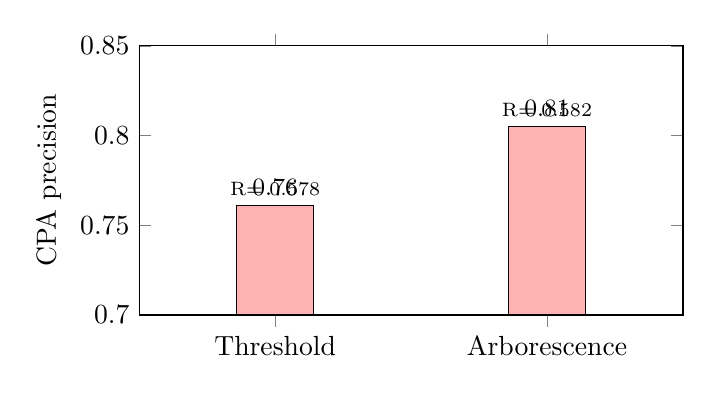
\begin{tikzpicture}
\begin{axis}[
    width=0.7\linewidth, height=5cm,
    ybar,
    bar width=28pt,
    ymin=0.70, ymax=0.85,
    ylabel={CPA precision},
    symbolic x coords={Threshold, Arborescence},
    xtick=data,
    nodes near coords,
    every node near coord/.append style={font=\small},
    enlarge x limits=0.5,
]
\addplot[fill=red!30] coordinates {(Threshold,0.761) (Arborescence,0.805)};
% annotate equal-recall context
\node[anchor=south, font=\scriptsize] at (axis cs:Threshold,0.761) {R$=0.578$};
\node[anchor=south, font=\scriptsize] at (axis cs:Arborescence,0.805) {R$=0.582$};
\end{axis}
\end{tikzpicture}

% Caption guidance (place when included): identical FLINT per-link scores; the only
% change is the decoder. The maximum-weight arborescence (one parent per column, no
% cycles) lifts PRECISION 0.761 -> 0.805 at unchanged recall -- the same global
% consistency GRAMS+'s Steiner tree provides, here from a textbook graph algorithm.
 inside a figure env.
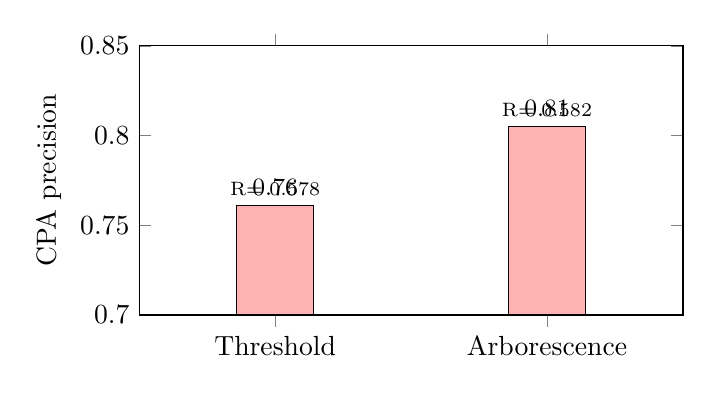
\begin{tikzpicture}
\begin{axis}[
    width=0.7\linewidth, height=5cm,
    ybar,
    bar width=28pt,
    ymin=0.70, ymax=0.85,
    ylabel={CPA precision},
    symbolic x coords={Threshold, Arborescence},
    xtick=data,
    nodes near coords,
    every node near coord/.append style={font=\small},
    enlarge x limits=0.5,
]
\addplot[fill=red!30] coordinates {(Threshold,0.761) (Arborescence,0.805)};
% annotate equal-recall context
\node[anchor=south, font=\scriptsize] at (axis cs:Threshold,0.761) {R$=0.578$};
\node[anchor=south, font=\scriptsize] at (axis cs:Arborescence,0.805) {R$=0.582$};
\end{axis}
\end{tikzpicture}

% Caption guidance (place when included): identical FLINT per-link scores; the only
% change is the decoder. The maximum-weight arborescence (one parent per column, no
% cycles) lifts PRECISION 0.761 -> 0.805 at unchanged recall -- the same global
% consistency GRAMS+'s Steiner tree provides, here from a textbook graph algorithm.
 inside a figure env.
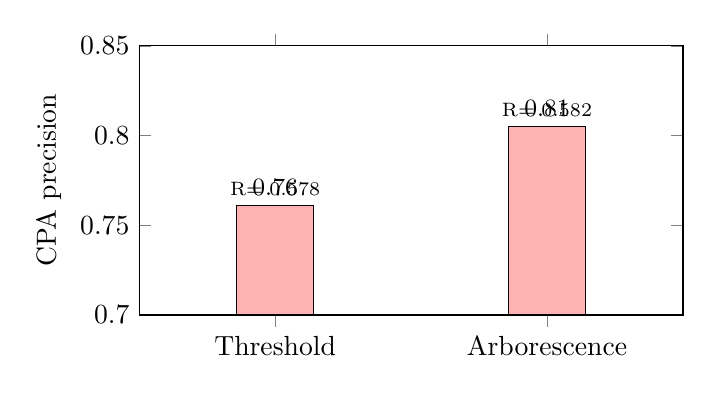
\begin{tikzpicture}
\begin{axis}[
    width=0.7\linewidth, height=5cm,
    ybar,
    bar width=28pt,
    ymin=0.70, ymax=0.85,
    ylabel={CPA precision},
    symbolic x coords={Threshold, Arborescence},
    xtick=data,
    nodes near coords,
    every node near coord/.append style={font=\small},
    enlarge x limits=0.5,
]
\addplot[fill=red!30] coordinates {(Threshold,0.761) (Arborescence,0.805)};
% annotate equal-recall context
\node[anchor=south, font=\scriptsize] at (axis cs:Threshold,0.761) {R$=0.578$};
\node[anchor=south, font=\scriptsize] at (axis cs:Arborescence,0.805) {R$=0.582$};
\end{axis}
\end{tikzpicture}

% Caption guidance (place when included): identical FLINT per-link scores; the only
% change is the decoder. The maximum-weight arborescence (one parent per column, no
% cycles) lifts PRECISION 0.761 -> 0.805 at unchanged recall -- the same global
% consistency GRAMS+'s Steiner tree provides, here from a textbook graph algorithm.
 inside a figure env.
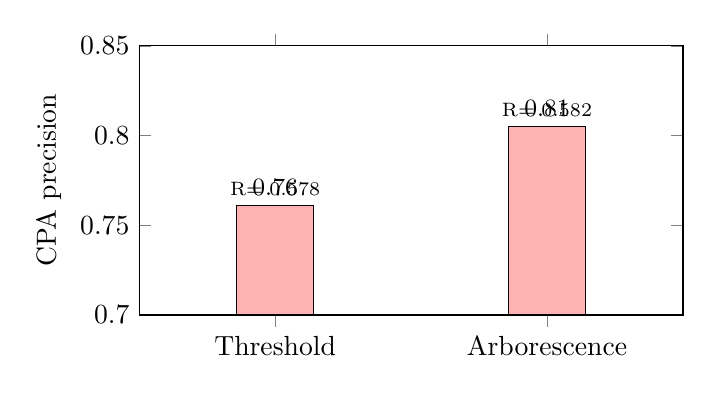
\begin{tikzpicture}
\begin{axis}[
    width=0.7\linewidth, height=5cm,
    ybar,
    bar width=28pt,
    ymin=0.70, ymax=0.85,
    ylabel={CPA precision},
    symbolic x coords={Threshold, Arborescence},
    xtick=data,
    nodes near coords,
    every node near coord/.append style={font=\small},
    enlarge x limits=0.5,
]
\addplot[fill=red!30] coordinates {(Threshold,0.761) (Arborescence,0.805)};
% annotate equal-recall context
\node[anchor=south, font=\scriptsize] at (axis cs:Threshold,0.761) {R$=0.578$};
\node[anchor=south, font=\scriptsize] at (axis cs:Arborescence,0.805) {R$=0.582$};
\end{axis}
\end{tikzpicture}

% Caption guidance (place when included): identical FLINT per-link scores; the only
% change is the decoder. The maximum-weight arborescence (one parent per column, no
% cycles) lifts PRECISION 0.761 -> 0.805 at unchanged recall -- the same global
% consistency GRAMS+'s Steiner tree provides, here from a textbook graph algorithm.
